\documentclass[fleqn,11pt]{article}

\usepackage[letterpaper,margin=0.75in]{geometry}

\usepackage{amsmath}
\usepackage{booktabs}
\usepackage{graphicx}
\usepackage{listings}

\setlength{\parindent}{1.4em}

\begin{document}

\lstset{
  language=Python,
  basicstyle=\small,          % print whole listing small
  keywordstyle=\bfseries,
  identifierstyle=,           % nothing happens
  commentstyle=,              % white comments
  stringstyle=\ttfamily,      % typewriter type for strings
  showstringspaces=false,     % no special string spaces
  numbers=left,
  numberstyle=\tiny,
  numbersep=5pt,
  frame=tb,
}

\title{Network Simulation (Lab 1) Report}

\author{Luke Dickinson}

\date{1/25/2017}

\maketitle

\section{Introduction}

In order to measure the way a basic network performs, we used a network simulator called Bene to simulate a number of different situations. In each of these situations, we will show how the simulation is set up, what the simulation resulted to, and alternate calculations to show that the result from the simulation is correct.
\subsubsection{Terms and Abbreviations }

In order to increase readability, abbreviations will be used throughout the paper. The following terms may be use in the abbreviated form:
\begin{align*}
Packet &= p\\
Node &= n\\
CreationTime &= cTime\\
ProcessingDelay &= procDelay\\
PropagationDelay &= propDelay\\
TransmissionDelay &= tDelay\\
QueueingDelay &= qDelay\\
\end{align*}

\section{Two Nodes}
This section includes a network that consisting of 2 nodes. The setup required for the simulations in this section is the same for each case. To setup the simulation, we first reset the scheduler for the simulation. Next, we set up the network by create a Network object by passing a network configuration file (which will be described in each simulation). After that, we set up the route information between the nodes. Finally, we setup a handler to print out information about packets received at node$_2$. The following code snippet performs the setup:
\begin{lstlisting}
# parameters
Sim.scheduler.reset()

# setup network
net = Network('lab1-onehopX.txt')

# setup routes
n1 = net.get_node('n1')
n2 = net.get_node('n2')
n1.add_forwarding_entry(address=n2.get_address('n1'), link=n1.links[0])
n2.add_forwarding_entry(address=n1.get_address('n2'), link=n2.links[0])

# setup app
d = DelayHandler()
net.nodes['n2'].add_protocol(protocol="delay", handler=d)
\end{lstlisting}

 \subsection{First simulation of a two node network}
\subsubsection{Simulation configuration}
For our first simulation of a two node network, we set the bandwidth between the nodes to 1 Mbps, and set the propagation delay between the nodes to 1 second. We send a single packet of size 1000 bytes from one node to the other at time set to 0 seconds. To do this we use the following configuration file:

\begin{lstlisting}
# n1 -- n2
n1 n2
n2 n1

# link configuration
n1 n2 1Mbps 1000ms
n2 n1 1Mbps 1000ms
\end{lstlisting}

This configuration file above is called 'lab1-onehopA.txt.' This is to be inserted into our Network constructor referred to above.
Once the network is set up, we will send our single packet to node$_2$ and then run the simulation. This is shown in the following code snippet:    

\begin{lstlisting}
#send packet(s)
p = Packet(destination_address=n2.get_address('n1'), \\
	ident=1, protocol='delay', length=1000)
Sim.scheduler.add(delay=0, event=p, handler=n1.send_packet)

# run the simulation
Sim.scheduler.run()
\end{lstlisting}

\subsubsection{Output of the simulation}
\begin{lstlisting}
(1.008, 1, 0, 1.008, 0.008, 1.0, 0)
\end{lstlisting}
This output shows that the first packet was created at 0 seconds, its identifier was 1, and the time it was received by node$_2$ was at 1.008 seconds.

\subsubsection{Verifying calculations}

We are able to calculate the time our packet is received at node$_2$ by adding the creation time of the packet, the processing delay, propagation delay, transmission delay, and queueing delay for this packet. In our simulation we are assuming that processing delay is 0. In situations of only a single packet, there is no queueing delay.

\begin{align*}
cTime_{p1} &= 0\,seconds\\
procDelay &= 0\,seconds\\
propDelay_{n1} &= 1\,second\\
tDelay_{p1\,at\,n1} &=  \frac{size\,of\,the\,packet} {link\,rates}\\
&= \frac{1000\,bytes} {1\,Mbps}\\
&=  \frac{8000\,bits} {1\,Mbps}\\
&= 0.008\,seconds\\
qDelay_{p1\,at\,n1} &= 0\,seconds\\
\\
Time\,Packet_{1}\,Is\,Received\,At\,Node_{2} &= \,cTime_{p1} + procDelay + propDelay_{n1} +\\
&\,\,\,\,\,\,\,\, + tDelay_{p1\,at\,n1} + qDelay_{p1\,at\,n1} \\
&= 0 + 0 + 1 + 0.008 + 0 \\
&= 1.008
\end{align*}

From our calculations we see that packet$_1$ is received at node$_2$ at 1.008 seconds, which matches our simulation.

 \subsection{Second simulation of a two node network}
\subsubsection{Simulation configuration}
For our second simulation of a two node network, we set the bandwidth between the nodes to 100 bps, and set the propagation delay between the nodes to 10 milliseconds. We send a single packet of size 1000 bytes from one node to the other at time set to 0 seconds. To do this, we use the following configuration file:

\begin{lstlisting}
# n1 -- n2
#
n1 n2
n2 n1

# link configuration
n1 n2 100bps 10ms
n2 n1 100bps 10ms

\end{lstlisting}

This configuration file above is called 'lab1-onehopB.txt.' This is to be inserted into our Network constructor referred to above.
Once the network is set up, we will send our single packet to node$_2$ and then run the simulation. This is shown in the following code snippet:    

\begin{lstlisting}
#send packet(s)
p = Packet(destination_address=n2.get_address('n1'), \\
	ident=1, protocol='delay', length=1000)
Sim.scheduler.add(delay=0, event=p, handler=n1.send_packet)

# run the simulation
Sim.scheduler.run()
\end{lstlisting}

\subsubsection{Output of the simulation}
\begin{lstlisting}
(80.01, 1, 0, 80.01, 80.0, 0.01, 0)
\end{lstlisting}
This output shows that the first packet was created at 0 seconds, its identifier was 1, and the time it was received by node$_2$ was at 80.01 seconds.

\subsubsection{Verifying calculations}

We are able to calculate the time our packet is received at node$_2$ by adding the creation time of the packet, the processing delay, propagation delay, transmission delay, and queueing delay for this packet. In our simulation we are assuming that processing delay is 0. In situations of only a single packet, there is no queueing delay.

\begin{align*}
cTime_{p1} &= 0\,seconds\\
procDelay &= 0\,seconds\\
propDelay_{n1} &=10\,milliseconds\\
tDelay_{p1\,at\,n1} &=  \frac{size\,of\,the\,packet} {link\,rates}\\
&= \frac{1000\,bytes}{100\,bps}\\
&=  \frac{8000\,bits}{100\,bps}\\
&= 80\,seconds\\
qDelay_{p1\,at\,n1} &= 0\,seconds\\
\\
Time\,Packet_{1}\,Is\,Received\,At\,Node_{2} &= \,cTime_{p1} + procDelay + propDelay_{n1} +\\
&\,\,\,\,\,\,\,\, + tDelay_{p1\,at\,n1} + qDelay_{p1\,at\,n1} \\
&= 0 + 0 + 0.01 + 80 + 0 \\
&= 80.01 
\end{align*}

From our calculations we see that packet$_1$ is received at node$_2$ at 80.01 seconds, which matches our simulation.

 \subsection{Third simulation of a two node network}
\subsubsection{Simulation configuration}
For our third simulation of a two node network, we set the bandwidth between the nodes to 1 Mbps, and set the propagation delay between the nodes to 10 milliseconds. We send 3 packets of size 1000 bytes from one node to the other at time set to 0 seconds. Then we send a single packet of size 1000 bytes from one node to the other at time set to 2 seconds. To do this we use the following configuration file:

\begin{lstlisting}
# n1 -- n2
#
n1 n2
n2 n1

# link configuration
n1 n2 1Mbps 10ms
n2 n1 1Mbps 10ms

\end{lstlisting}

This configuration file above is called 'lab1-onehopC.txt.' This is to be inserted into our Network constructor referred to above.
Once the network is set up, we will send our packets to node$_2$ and then run the simulation. This is shown in the following code snippet:    

\begin{lstlisting}
#send packet(s)
p = Packet(destination_address=n2.get_address('n1'), \\
	ident=1, protocol='delay', length=1000)
Sim.scheduler.add(delay=0, event=p, handler=n1.send_packet)

p2 = Packet(destination_address=n2.get_address('n1'), \\
	ident=2, protocol='delay', length=1000)
Sim.scheduler.add(delay=0, event=p2, handler=n1.send_packet)

p3 = Packet(destination_address=n2.get_address('n1'), \\
	ident=3, protocol='delay', length=1000)
Sim.scheduler.add(delay=0, event=p3, handler=n1.send_packet)

p4 = Packet(destination_address=n2.get_address('n1'), \\
	ident=4, protocol='delay', length=1000)
Sim.scheduler.add(delay=2, event=p4, handler=n1.send_packet)    

# run the simulation
Sim.scheduler.run()
\end{lstlisting}

\subsubsection{Output of the simulation}
\begin{lstlisting}
(0.018000000000000002, 1, 0, 0.018000000000000002, 0.008, 0.01, 0)
(0.026000000000000002, 2, 0, 0.026000000000000002, 0.008, 0.01, 0.008)
(0.034, 3, 0, 0.034, 0.008, 0.01, 0.016)
(2.018, 4, 2.0, 0.017999999999999794, 0.008, 0.01, 0.0)

\end{lstlisting}
This output shows that the first packet was created at 0 seconds, its identifier was 1, and the time it was received by node$_2$ was at 0.018 seconds. The second packet was created at 0 seconds, its identifier was 2, and the time it was received by node$_2$ was at 0.0260 seconds. The third packet was created at 0 seconds, its identifier was 3, and the time it was received by node$_2$ was at 0.340 seconds. The fourth packet was created at 2 seconds, its identifier was 4, and the time it was received by node$_2$ was at 2.018 seconds.

\subsubsection{Verifying calculations}
We are able to calculate the time each of our packets are received at node$_2$ by adding the creation time of the packet, the processing delay, propagation delay, transmission delay, and queueing delay for a packet. In our simulation we are assuming that processing delay is 0. 

\paragraph{Calculating the time packet$_1$ is received at node$_2$ }
\begin{align*}
cTime_{p1} &= 0\,seconds\\
procDelay &= 0\,seconds\\
propDelay_{n1} &= 10\,milliseconds\\
tDelay_{p1\,at\,n1} &=  \frac{size\,of\,the\,packet} {link\,rates}\\
&= \frac{1000\,bytes} {1\,Mbps}\\
&=  \frac{8000\,bits} {1\,Mbps}\\
&= 0.008 \,seconds\\
qDelay_{pX\,at\,nY} &= k_{X}*(tDelay_{pX\,at\,nY} - tDelay_{packetX\,at\,n(Y-1)}) \\
&\text{where k$_X$ = the number of packets at node$_y$ when packet$_x$ arrives}\\
\\
k_{1} &= 0\\
&\text{Packet$_1$ is the first packet and will not enter a queue, so k$_1$ = 0} \\
qDelay_{p1\,at\,n1} &= k_{1}*(tDelay_{p1\,at\,n1} - tDelay_{p1\,at\,n(1-1)})\\
&= (0) (0.008 - 0) \\
&= 0 \\
\\
time\,packet_{1}\,is\,received\,at\,node_{2} &= \,cTime_{p1} + procDelay + propDelay_{n\,1} +\\
&\,\,\,\,\,\,\,\, + tDelay_{p\,1\,at\,n\,1} + qDelay_{p\,1\,at\,n\,1} \\
&= 0 + 0 + 0.01 + 0.008 + 0 \\
&= 0.018\\
\text{From our calculations we see that }
&\text{packet$_1$ is received at node$_2$ at 0.018 seconds,} \\
\text{which matches our simulation.}
\end{align*}

\paragraph{Calculating the time packet$_2$ is received at node$_2$ }
\begin{align*}
cTime_{p2} &= 0\,seconds\\
procDelay &= 0\,seconds\\
propDelay_{n1} &= 10\,milliseconds\\
&\text{As packet 1 and 2, are the same size, the value for}\\
&\text{tDelay$_{p1\,at\,n1}$ is the same as tDelay${_p2\,at\,n1}$}\\
&\text{So,}\\
tDelay_{p2\,at\,n1} &=  0.008 \,seconds\\
qDelay_{pX\,at\,nY} &= k_{X}*(tDelay_{pX\,at\,nY} - tDelay_{packetX\,at\,n(Y-1)}) \\
&\text{where k$_X$ = the number of packets at node$_y$ when packet$_x$ arrives}\\
\\
k_{2} &= 1\\
&\text{Packets 1, 2, and 3 arrive at node$_1$ at 0 seconds.}\\
&\text{When these are the these packets created,}\\
&\text{there are no other packets at node$_1$.}\\
&\text{As packet$_1$ is the only packet in front of packet$_2$, k$_2$ = 1.} \\
qDelay_{p2\,at\,n1} &= k_{2}*(tDelay_{p2\,at\,n1} - tDelay_{p2\,at\,n(1-1)})\\
&= (1) (0.008 - 0) \\
&= 0.008 \\
\\
time\,packet_{2}\,is\,received\,at\,node_{2} &= \,cTime_{p2} + procDelay + propDelay_{n\,1} +\\
&\,\,\,\,\,\,\,\, + tDelay_{p\,2\,at\,n\,1} + qDelay_{p\,2\,at\,n\,1} \\
&= 0 + 0 + 0.01 + 0.008 + 0.008 \\
&= 0.026\\
\text{From our calculations we see that }
&\text{packet$_2$ is received at node$_2$ at 0.026 seconds,} \\
\text{which matches our simulation.}
\end{align*}
\paragraph{Calculating the time packet$_3$ is received at node$_2$ }
\begin{align*}
cTime_{p3} &= 0\,seconds\\
procDelay &= 0\,seconds\\
propDelay_{n1} &= 10\,milliseconds\\
&\text{As packet 1 and 3 are the same size, the value for}\\
&\text{tDelay$_{p1\,at\,n1}$ is the same as tDelay${_{p3\,at\,n1}}$}\\
&\text{So,}\\
tDelay_{p3\,at\,n1} &=  0.008 \,seconds\\
qDelay_{pX\,at\,nY} &= k_{X}*(tDelay_{pX\,at\,nY} - tDelay_{packetX\,at\,n(Y-1)}) \\
&\text{where k$_X$ = the number of packets at node$_y$ when packet$_x$ arrives}\\
\\
k_{3} &= 2\\
&\text{Packets 1, 2, and 3 arrive at node$_1$ at 0 seconds.}\\
&\text{When these are the these packets created,}\\
&\text{there are no other packets at node$_1$.}\\
&\text{As packet$_1$ and packet$_2$ are the only packets in front of packet$_3$, k$_3$ = 2.} \\
qDelay_{p3\,at\,n1} &= k_{3}*(tDelay_{p3\,at\,n1} - tDelay_{p3\,at\,n(1-1)})\\
&= (2) (0.008 - 0) \\
&= 0.016 \\
\\
time\,packet_{3}\,is\,received\,at\,node_{2}  &= \,cTime_{p2} + procDelay + propDelay_{n\,1} +\\
&\,\,\,\,\,\,\,\, + tDelay_{p\,2\,at\,n\,1} + qDelay_{p\,2\,at\,n\,1} \\
&= 0 + 0 + 0.01 + 0.008 + 0.016 \\
&= 0.034\\
\text{From our calculations we see that }
&\text{packet$_3$ is received at node$_2$ at 0.034 seconds,} \\
\text{which matches our simulation.}
\end{align*}
\paragraph{Calculating the time packet$_4$ is received at node$_2$ }
\begin{align*}
cTime_{p4} &= 2\,seconds\\
procDelay &= 0\,seconds\\
propDelay_{n1} &= 10\,milliseconds\\
&\text{As packet 1 and 4 are the same size, the value for}\\
&\text{tDelay$_{p1\,at\,n1}$ is the same as tDelay$_{p4\,at\,n1}$}\\
&\text{So,}\\
tDelay_{p4\,at\,n1} &=  0.008 \,seconds\\
qDelay_{pX\,at\,nY} &= k_{X}*(tDelay_{pX\,at\,nY} - tDelay_{packetX\,at\,n(Y-1)}) \\
&\text{where k$_X$ = the number of packets at node$_y$ when packet$_x$ arrives}\\
\\
k_{3} &= 2\\
&\text{Packet$_ 4$ arrives at node$_1$ at 2 seconds.}\\
&\text{The packet previous to packet$_4$, packet$_3$, leaves node$_1$ at}\\
&\text{(packet$_3$ arrival time to node$_2$) - (propDelay$_{n1}$) =}\\
&\text{0.034 - 0.01 = 0.024 seconds. }\\
&\text{Because the previous packet to packet$_4$, packet$_3$, leaves node$_1$}\\
&\text{before packet$_4$ arrives, packet$_4$ does not enter the queue. So k = 0.} \\
qDelay_{p4\,at\,n1} &= k_{4}*(tDelay_{p4\,at\,n1} - tDelay_{p4\,at\,n(1-1)})\\
&= (0) (0.008 - 0) \\
&= 0 \\
\\
time\,packet_{4}\,is\,received\,at\,node_{2}  &= \,cTime_{p2} + procDelay + propDelay_{n\,1} +\\
&\,\,\,\,\,\,\,\, + tDelay_{p\,2\,at\,n\,1} + qDelay_{p\,2\,at\,n\,1} \\
&= 2 + 0 + 0.01 + 0.008 + 0 \\
&= 2.018\\
\text{From our calculations we see that }
&\text{packet$_4$ is received at node$_2$ at 2.018 seconds,} \\
\text{which matches our simulation.}
\end{align*}
\section{Three Nodes}
This section includes a network that consisting of 3 nodes. The setup required for the simulations in this section is the same for each case. To setup the simulation, we first reset the scheduler for the simulation. Next, we set up the network by create a Network object by passing a network configuration file (which will be described in each simulation). After that, we set up the route information between the nodes. Finally, we setup a handler to print out information about packets received at node$_3$. The following code snippet performs the setup:
\begin{lstlisting}
# parameters
Sim.scheduler.reset()

# setup network
net = Network('lab1-twohopX.txt')

# setup routes
n1 = net.get_node('n1')
n2 = net.get_node('n2')
n3 = net.get_node('n3')
n1.add_forwarding_entry(address=n2.get_address('n1'), link=n1.links[0])
n1.add_forwarding_entry(address=n3.get_address('n2'), link=n1.links[0])
n2.add_forwarding_entry(address=n1.get_address('n2'), link=n2.links[0])
n2.add_forwarding_entry(address=n3.get_address('n2'), link=n2.links[1])
n3.add_forwarding_entry(address=n2.get_address('n3'), link=n3.links[0])
n3.add_forwarding_entry(address=n1.get_address('n2'), link=n3.links[0])

# setup app
d = DelayHandler()
net.nodes['n3'].add_protocol(protocol="delay", handler=d)
\end{lstlisting}
\subsection{First simulation of a three node network - Part 1}
\subsubsection{Simulation configuration}
For our first simulation of a three node network, we set the bandwidth between the node$_1$ and node$_2$ to 1 Mbps, the bandwidth from node$_2$ to node$_3$ to 1 Mbps, set the propagation delay between the node$_1$ and node$_2$ to 100 milliseconds, and set the propagation delay between the node$_2$ to node$_3$ to 100 milliseconds. We send a 1000 packets, each 1000 bytes in size through the network with the source being node$_1$ and the destination being node$_3$. To do this we use the following configuration file:
\begin{lstlisting}
# n1 -- n2 -- n3
n1 n2
n2 n1
n2 n3
n3 n2
# link configuration
n1 n2 1Mbps 100ms
n2 n1 1Mbps 100ms
n2 n3 1Mbps 100ms
n3 n2 1Mbps 100ms
\end{lstlisting}
This configuration file above is called 'lab1-twohopA.txt.' This is to be inserted into our Network constructor referred to above.
Once the network is set up, we will send a single file in 1000 packets to node three and then run the simulation. In order to avoid queueing issues (like overflowing the simulated queue), we will control the time each packet is sent so that each packet will be begin its process as its previous packet leaves node$_1$. This is shown in the following code snippet:    

\begin{lstlisting}
trasmissionDelay = 8.0/1000.0    
# send packets
for i in range(1,1001):
    calculatedDelay = (i-1) * trasmissionDelay
    p = Packet(destination_address=n3.get_address('n2'), ident=i, protocol='delay',
	length=1000)
    Sim.scheduler.add(delay=calculatedDelay, event=p, handler=n1.send_packet)
# run the simulation
Sim.scheduler.run() 
\end{lstlisting}
\subsubsection{Output of the simulation}
Last 5 entries:
\begin{lstlisting}
(8.176000000000007, 996, 7.96, 0.2160000000000073, 0.016, 0.2, 6.217248937900877e-15)
(8.184000000000006, 997, 7.968, 0.2160000000000064, 0.016, 0.2, 6.217248937900877e-15)
(8.192000000000007, 998, 7.976, 0.2160000000000073, 0.016, 0.2, 6.217248937900877e-15)
(8.200000000000006, 999, 7.984, 0.2160000000000064, 0.016, 0.2, 6.217248937900877e-15)
(8.208000000000007, 1000, 7.992, 0.2160000000000073, 0.016, 0.2, 6.217248937900877e-15)
\end{lstlisting}
The entire file is transfered when the last packet arrives at node$_3$. This output shows that the last packet arrived at node$_3$ at 8.208 seconds. We can see that the true transmission delay dominates as the packet creation time (used to mimic transmission delay from the node$_1$) which is 7.992, plus the recorded transmission delay, which is 0.016, equals 8.008 seconds. This is much greater than the next closest delay, which is propagation delay, at 0.2 seconds.
\subsubsection{Verifying calculations}
We are able to calculate the time our file is received at node$_3$ by calculating the time our last packet, packet$_{1000}$, is received at node $_3$. We calculate the time it takes for packet$_{1000}$ to reach node$_2$ by adding the creation time, processing delay, propagation delay, transmission delay, and queueing delay for packet$_{1000}$ going to node$_2$. We then can calculate the total time it takes to get to node$_3$ by adding the arrival time to node$_2$ for packet$_{1000}$ to the processing delay, propagation delay, transmission delay, and queueing delay for packet$_{1000}$ going to node$_3$. In our simulation we are assuming that processing delay is 0. As we are throttling our creation time of each packet, we will have no queueing delay at node$_1$. Also, because all of the links in our network are the same speed, every time a packet reaches a node the previous node would have just left. Therefore, there is no queuing delay for node$_2$  either.

\paragraph{Calculating the time packet$_{1000}$ is received at node$_2$ }
\begin{align*}
tDelay_{p1000\,at\,n1} &=  \frac{size\,of\,the\,packet} {link\,rates}\\
&= \frac{1000\,bytes} {1\,Mbps}\\
&=  \frac{8000\,bits} {1\,Mbps}\\
&= 0.008 \,seconds\\
cTime_{p1000} &= (1000-1) *tDelay_{n1}\,seconds\\
&= (999) *(0.008)\,seconds\\
&= 7.992\,seconds\\
procDelay &= 0\,seconds\\
propDelay_{n1} &= 0.1\,seconds\\
qDelay_{p1000\,at\,n1} &= 0\\
time\,packet_{1000}\,is\,received\,at\,node_{2} &= \,cTime_{p1000} + procDelay + propDelay_{n\,1} +\\
&\,\,\,\,\,\,\,\, + tDelay_{p\,1000,at\,n\,1} + qDelay_{p\,1000\,at\,n\,1}\\
&= 7.992 + 0 + 0.1 + 0.008 + 0\,seconds\\
&= 8.1\,seconds
\end{align*}

\paragraph{Calculating the time packet$_{1000}$ is received at node$_3$ }
\begin{align*}
tDelay_{p1000\,at\,n2} &=  \frac{size\,of\,the\,packet} {link\,rates}\\
&= \frac{1000\,bytes} {1\,Mbps}\\
&=  \frac{8000\,bits} {1\,Mbps}\\
&= 0.008 \,seconds\\
time\,packet_{1000}\,is\,received\,at\,node_{2} &= 8.1\,seconds\\
procDelay &= 0\,seconds\\
propDelay_{n2} &= 0.1\,seconds\\
qDelay_{p1000\,at\,n2} &= 0\\
time\,packet_{1000}\,is\,received\,at\,node_{3} &= \,time\,packet_{1000}\,is\,received\,at\,node_{2} + \\
&\,\,\,\,\,\,\,\, + procDelay + propDelay_{n\,2} + tDelay_{p\,1000\,at\,n\,2} \\
&\,\,\,\,\,\,\,\, + qDelay_{p\,1000\,at\,n\,2}\\
&= 8.1 + 0 + 0.1 + 0.008 + 0\,seconds\\
&= 8.208\,seconds \\
\text{From our calculations we see that }
&\text{packet$_{1000}$ is received at node$_3$ at 8.208 seconds,} \\
\text{which matches our simulation.}
\end{align*}
\subsection{First simulation of a three node network - Part 2}
\subsubsection{Simulation configuration}
We repeated our first simulation of a three node network, but this time we set the bandwidth between the node$_1$  and node$_2$  to 1 Gbps, the bandwidth from node$_2$  and node$_3$ to 1 Gbps. We still set the propagation delay between the node$_1$  and node$_2$ to 100 milliseconds, and set the propagation delay between the node$_2$  and node$_3$ to 100 milliseconds. We send a 1000 packets, each 1000 bytes in size through the network with the source being node$_1$ and the destination being node$_3$. To do this we use the following configuration file:
\begin{lstlisting}
# n1 -- n2 -- n3
n1 n2
n2 n1 n3
n3 n2

# link configuration
n1 n2 1Gbps 100ms
n2 n1 1Gbps 100ms
n2 n3 1Gbps 100ms
n3 n2 1Gbps 100ms
\end{lstlisting}
This configuration file above is called 'lab1-twohopA2.txt.' This is to be inserted into our Network constructor referred to above.
Once the network is set up, we will send a single file in 1000 packets to node three and then run the simulation. In order to avoid queueing issues (like overflowing the simulated queue), we will control the time each packet is sent so that each packet will be begin its process as its previous packet leaves node$_1$. This is shown in the following code snippet:    

\begin{lstlisting}
#8kbit/1Gbps = 8kbit/1000000kbps
trasmissionDelay = 8.0/1000000.0 
# send packets
for i in range(1,1001):
    calculatedDelay = (i-1) * trasmissionDelay
    p = Packet(destination_address=n3.get_address('n2'), ident=i, protocol='delay', 
	length=1000)
    Sim.scheduler.add(delay=calculatedDelay, event=p, handler=n1.send_packet)
# run the simulation
Sim.scheduler.run() 
\end{lstlisting}
\subsubsection{Output of the simulation}
Last 5 entries:
\begin{lstlisting}
(0.20797600000000013, 996, 0.00796, 0.20001600000000014, 1.6e-05, 0.2, 
	1.3010426069826053e-16)
(0.2079840000000001, 997, 0.007968, 0.2000160000000001, 1.6e-05, 0.2,
	1.3010426069826053e-16)
(0.20799200000000012, 998, 0.007976, 0.2000160000000001, 1.6e-05, 0.2, 
	1.2836953722228372e-16)
(0.20800000000000013, 999, 0.007984, 0.20001600000000014, 1.6e-05, 0.2, 
	1.2836953722228372e-16)
(0.20800800000000014, 1000, 0.007991999999999999, 0.20001600000000014, 1.6e-05, 0.2, 
	1.2836953722228372e-16)
\end{lstlisting}
The entire file is transfered when the last packet arrives at node$_3$. This output shows that the last packet arrived at node$_3$ at about 0.208008 seconds. We can see that the true transmission delay is the packet creation time (used to mimic transmission delay from the node$_1$) which is about 0.007992 seconds, plus the recorded transmission delay, which is 0.000016, equals 0.008008 seconds. This time we can see that propagration delay is much higher and is the dominate delay at 0.2 seconds.
\subsubsection{Verifying calculations}
We are able to calculate the time our file is received at node$_3$ by calculating the time our last packet, packet$_{1000}$, is received at node $_3$. We calculate the time it takes for packet$_{1000}$ to reach node$_2$ by adding the creation time, processing delay, propagation delay, transmission delay, and queueing delay for packet$_{1000}$ going to node$_2$. We then can calculate the total time it takes to get to node$_3$ by adding the arrival time to node$_2$ for packet$_{1000}$ to the processing delay, propagation delay, transmission delay, and queueing delay for packet$_{1000}$ going to node$_3$. In our simulation we are assuming that processing delay is 0. As we are throttling our creation time of each packet, we will have no queueing delay at node$_1$. Also, because all of the links in our network are the same speed, every time a packet reaches a node the previous node would have just left. Therefore, there is no queuing delay for node$_2$ either.

\paragraph{Calculating the time packet$_{1000}$ is received at node$_2$ }
\begin{align*}
tDelay_{p1000\,at\,n1} &=  \frac{size\,of\,the\,packet} {link\,rates}\\
&= \frac{1000\,bytes} {1\,Gbps}\\
&=  \frac{8000\,bits} {1\,Gbps}\\
&= 0.000008 \,seconds\\
cTime_{p1000} &= (1000-1) *tDelay_{n1}\,seconds\\
&= (999) *(0.000008)\,seconds\\
&= 0.007992\,seconds\\
procDelay &= 0\,seconds\\
propDelay_{n1} &= 0.1\,seconds\\
qDelay_{p1000\,at\,n1} &= 0\\
time\,packet_{1000}\,is\,received\,at\,node_{2} &= \,cTime_{p1000} + procDelay + propDelay_{n\,1} +\\
&\,\,\,\,\,\,\,\, + tDelay_{p\,1000\,at\,n\,1} + qDelay_{p\,1000\,at\,n\,1}\\
&= 0.007992 + 0 + 0.1 + 0.000008 + 0\,seconds\\
&= 0.108\,seconds
\end{align*}

\paragraph{Calculating the time packet$_{1000}$ is received at node$_3$ }
\begin{align*}
tDelay_{p1000\,at\,n2} &=  \frac{size\,of\,the\,packet} {link\,rates}\\
&= \frac{1000\,bytes} {1\,Mbps}\\
&=  \frac{8000\,bits} {1\,Mbps}\\
&= 0.000008 \,seconds\\
time\,packet_{1000}\,is\,received\,at\,node_{2} &= 0.108\,seconds\\
procDelay &= 0\,seconds\\
propDelay_{n2} &= 0.1\,seconds\\
qDelay_{p1000\,at\,n2} &= 0\\
time\,packet_{1000}\,is\,received\,at\,node_{3} &= \,time\,packet_{1000}\,is\,received\,at\,node_{2} + \\
&\,\,\,\,\,\,\,\, + procDelay + propDelay_{n\,2} + tDelay_{p\,1000\,at\,n\,2} \\
&\,\,\,\,\,\,\,\, + qDelay_{p\,1000\,at\,n\,2}\\
&= 0.108 + 0 + 0.1 + 0.000008 + 0\,seconds\\
&= 0.208008\,seconds \\
\text{From our calculations we see that }
&\text{packet$_{1000}$ is received at node$_3$ at 0.208008 seconds,} \\
\text{which matches our simulation.}
\end{align*}
\subsection{Second simulation of a three node network}
\subsubsection{Simulation configuration}
For our second simulation of a three node network, we set the bandwidth between the node$_1$ and node$_2$ to 1 Mbps, the bandwidth from node$_2$ and node$_3$  to 256 Kbps, set the propagation delay between the node$_1$ and node$_2$  to 100 milliseconds, and set the propagation delay between the node$_2$ and node$_3$ to 100 milliseconds. We send a 1000 packets, each 1000 bytes in size through the network with the source being node$_1$ and the destination being node$_3$. To do this we use the following configuration file:
\begin{lstlisting}
# n1 -- n2 -- n3
n1 n2
n2 n1 n3
n3 n2

# link configuration
n1 n2 1Mbps 100ms
n2 n1 1Mbps 100ms
n2 n3 256Kbps 100ms
n3 n2 256Kbps 100ms
\end{lstlisting}
This configuration file above is called 'lab1-twohopB.txt.' This is to be inserted into our Network constructor referred to above.
Once the network is set up, we will send a single file in 1000 packets to node three and then run the simulation. In order to avoid queueing issues (like overflowing the simulated queue), we will control the time each packet is sent so that each packet will be begin its process as its previous packet leaves node$_1$. This is shown in the following code snippet:    

\begin{lstlisting}
trasmissionDelay = 8.0/1000.0    
# send packets
for i in range(1,1001):
    calculatedDelay = (i-1) * trasmissionDelay
    p = Packet(destination_address=n3.get_address('n2'), ident=i, protocol='delay', length=1000)
    Sim.scheduler.add(delay=calculatedDelay, event=p, handler=n1.send_packet)
# run the simulation
Sim.scheduler.run() 
\end{lstlisting}
\subsubsection{Output of the simulation}
Last 5 entries:
\begin{lstlisting}
(31.333000000000002, 996, 7.96, 23.373, 0.03925, 0.2, 23.13375)
(31.364250000000002, 997, 7.968, 23.396250000000002, 0.03925, 0.2, 23.157000000000004)
(31.395500000000002, 998, 7.976, 23.419500000000003, 0.03925, 0.2, 23.18025)
(31.426750000000002, 999, 7.984, 23.442750000000004, 0.03925, 0.2, 23.203500000000002)
(31.458000000000002, 1000, 7.992, 23.466, 0.03925, 0.2, 23.226750000000003)
\end{lstlisting}
The entire file is transfered when the last packet arrives at node$_3$. This output shows that the last packet arrived at node$_3$ at about 31.458 seconds.
\subsubsection{Verifying calculations}
We are able to calculate the time our file is received at node$_3$ by calculating the time our last packet, packet$_{1000}$, is received at node $_3$. We calculate the time it takes for packet$_{1000}$ to reach node$_2$ by adding the creation time, processing delay, propagation delay, transmission delay, and queueing delay for packet$_{1000}$ going to node$_2$. We then can calculate the total time it takes to get to node$_3$ by adding the arrival time to node$_2$ for packet$_{1000}$ to the processing delay, propagation delay, transmission delay, and queueing delay for packet$_{1000}$ going to node$_3$. In our simulation we are assuming that processing delay is 0. As we are throttling our creation time of each packet, we will have no queueing delay at node$_1$. There will be queueing delay at node$_2$ because the bandwidth from node$_2$ to node$_3$ is less than the bandwidth from node$_1$ to node$_2$. Because there are no gaps in the streaming of our 1000 packets, we are able to use a simpler formula to calculate queueing delay. The formula will be shown below is as follows:

\begin{align*}
qDelay_{pk\,at\,n2} = (k - 1) (tDelay_{pk\,at\,n2} - tDelay_{pk\,at\,n1})
\end{align*}

\paragraph{Calculating the time packet$_{1000}$ is received at node$_2$ }
\begin{align*}
tDelay_{p1000\,at\,n1} &=  \frac{size\,of\,the\,packet} {link\,rates}\\
&= \frac{1000\,bytes} {1\,Mbps}\\
&=  \frac{8000\,bits} {1\,Mbps}\\
&= 0.008 \,seconds\\
cTime_{p1000} &= (1000-1) *tDelay_{n1}\,seconds\\
&= (999) *(0.008)\,seconds\\
&= 7.992\,seconds\\
procDelay &= 0\,seconds\\
propDelay_{n1} &= 0.1\,seconds\\
qDelay_{p1000\,at\,n1} &= 0\\
time\,packet_{1000}\,is\,received\,at\,node_{2} &= \,cTime_{p1000} + procDelay + propDelay_{n\,1} +\\
&\,\,\,\,\,\,\,\, + tDelay_{p\,1000\,at\,n\,1} + qDelay_{p\,1000\,at\,n\,1}\\
&= 7.992 + 0 + 0.1 + 0.008 + 0\,seconds\\
&= 8.1\,seconds
\end{align*}

\paragraph{Calculating the time packet$_{1000}$ is received at node$_3$ }
\begin{align*}
tDelay_{p1000\,at\,n2} &=  \frac{size\,of\,the\,packet} {link\,rates}\\
&= \frac{1000\,bytes} {256\,Kbps}\\
&=  \frac{8000\,bits} {256\,Kbps}\\
&= 0.03125 \,seconds\\
time\,packet_{1000}\,is\,received\,at\,node_{2} &= 8.1\,seconds\\
procDelay &= 0\,seconds\\
propDelay_{n2} &= 0.1\,seconds\\
\\
qDelay_{p1000\,at\,n2} &= (k - 1) (tDelay_{p1000\,at\,n2} - tDelay_{p1000\,at\,n1}\\
&=(1000 - 1) (0.03125\,seconds - 0.008\,seconds)\\
&=23.22675 \\
time\,packet_{1000}\,is\,received\,at\,node_{3} &= \,time\,packet_{1000}\,is\,received\,at\,node_{2} + \\
&\,\,\,\,\,\,\,\, + procDelay + propDelay_{n\,2} + tDelay_{p\,1000\,at\,n\,2} \\
&\,\,\,\,\,\,\,\, + qDelay_{p\,1000\,at\,n\,2}\\
&= 8.1 + 0 + 0.1 + 0.03125 + 23.22675\,seconds\\
&= 31.458\,seconds \\
\text{From our calculations we see that }
&\text{packet$_{1000}$ is received at node$_3$ at 31.458 seconds,} \\
\text{which matches our simulation.}
\end{align*}

\section{Queueing Theory}
In this section, we explore how well our simulation matches up to queueing theory. We will simulate a M/D/1 queue. The "M" means that there is an exponential distribution of arrival times. The "D" means there is a deterministic service time. The "1" means that there is only 1 queue. It is expected that as our utilization percentage of our maximum rate approaches 100\%, the average queueing delay will go to infinity.

Our simulator streams packets in between two nodes for 10 seconds. The rate that the packets are created and sent is determined by passing a utilization percentage of the maximum rate into a random exponential distribution function. We chose a number of different utilization percentages. We ran these utilization percentages through our experiment, and then graphed the average queueing delay for each utilization percentage. 

We also graphed the theoretical values for each of the utilization percentages using the following formula:

\begin{align*}
w &= \frac{1} {2u} * \frac{p} {1-p} \\
&where\,u\,=\,service\,rate\\
&and\,where\,p\,=\,utilization\,percentage
\end{align*}

\subsection{Simulation configuration}
 To setup the simulation, we first reset the scheduler for the simulation. Next, we set up the network by create a Network object by passing a network configuration file (which will be described below). After that, we set up the route information between the nodes. Finally, we setup a handler to print out information about packets received at node$_2$ to a file.  The following code snippet performs the setup:
\begin{lstlisting}
    # parameters
    Sim.scheduler.reset()

    # setup network
    net = Network('../networks/one-hop.txt')

    # setup routes
    n1 = net.get_node('n1')
    n2 = net.get_node('n2')
    n1.add_forwarding_entry(address=n2.get_address('n1'), link=n1.links[0])
    n2.add_forwarding_entry(address=n1.get_address('n2'), link=n2.links[0])

    # setup app
    d = DelayHandler()
    net.nodes['n2'].add_protocol(protocol="delay", handler=d)

\end{lstlisting}

Our simulated network had two nodes. We set the bandwidth between the nodes to 1 Mbps, and set the propagation delay between the nodes to 1 second. To do this we use the following configuration file:

\begin{lstlisting}
# n1 -- n2
n1 n2
n2 n1

# link configuration
n1 n2 1Mbps 1000ms
n2 n1 1Mbps 1000ms
\end{lstlisting}

This configuration file above is called 'lab1-queueingtheory.txt.' This is to be inserted into our Network constructor referred to above.
Once the network is set up, we then need to set up a way to continually send packets as we need them. This can be done with a Generator class. This class generates packets based on the load parameter passed in and the random.expovariate function. This shown in the following code snippet: 
\begin{lstlisting}
class Generator(object):
def __init__(self, node, destination, load, duration):
	self.node = node
	self.load = load
	self.destination = destination
	self.duration = duration
	self.start = 0
	self.ident = 1

def handle(self, event):
	# quit if done
	now = Sim.scheduler.current_time()
	if (now - self.start) > self.duration:
		return

	# generate a packet
	self.ident += 1
	p = Packet(destination_address=self.destination, ident=self.ident, 
		protocol='delay', length=1000)
	Sim.scheduler.add(delay=0, event=p, handler=self.node.send_packet)
	# schedule the next time we should generate a packet
	Sim.scheduler.add(delay=random.expovariate(self.load), event='generate', 
		handler=self.handle)
\end{lstlisting}

Lastly, we need to generate our load parameter and start our simulator. First, we calculate the maximum rate our link can handle (in packets/second), which is 1Mbps/8Kbit packet size. Then we multiply this value by the utilization percentage chosen for the experiment. After we have this value, we create our Generator object by passing in the source node, destination node, the load value, and 10 seconds of duration time. Lastly, we start the simulation. This is shown in the following code snippet:
\begin{lstlisting}
# setup packet generator
destination = n2.get_address('n1')
max_rate = 1000000 // (1000 * 8)
myLoadPercent = 98

load = myLoadPercent/100.0 * max_rate
g = Generator(node=n1, destination=destination, load=load, duration=10)
Sim.scheduler.add(delay=0, event='generate', handler=g.handle)

# run the simulation
Sim.scheduler.run()
\end{lstlisting}
\subsection{Experiment}
In our experiement we used the following utilization values: 10\%, 20\%, 30\%, 40\%, 50\%, 60\%, 70\%, 80\%, 90\%, 95\%, and 98\%.

For each utilization value, we recorded the queueing time for each packet sent. The number of packets sent varied from about 100 to 1000 depending on how high the utilization was. We then calculated the average queueing delay for each utilization value. The averages were created by running the data through a python script. The averages were as following:
\begin{align*}
10\%&=0.000246186799194\,seconds\\
20\%&=0.000744426315041\,seconds\\
30\%&=0.00180887562312\,seconds\\
40\%&=0.00207776042834\,seconds\\
50\%&=0.00370991960505\,seconds\\
60\%&=0.00617988242069\,seconds\\
70\%&=0.0083786921238\,seconds\\
80\%&=0.0148861562441\,seconds\\
90\%&=0.0422212596784\,seconds\\
95\%&=0.0289565539489\,seconds\\
98\%&=0.0457814929168\,seconds
\end{align*}

As you can see from our data, the random exponential distribution function showed blips in our data. This is seen in that 90\% had a high queuing delay than 95\%. Nevertheless, it can be seen that as the utilization increases so does the queueing delay.

In the graph below, we graphed our experimental data in blue and the theoretical data in green. The theoretical data was created by using the function described above. As 

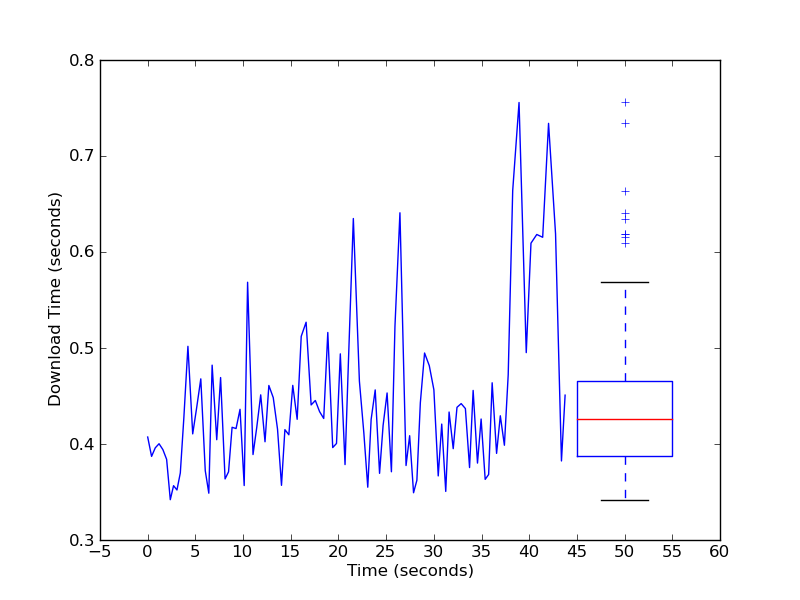
\includegraphics[width=11cm]{graphs/download-combined}

you can see from the graph, the ...


\end{document}
